% figures/normalization-before-after.tex
\documentclass[11pt]{article}
\usepackage[margin=1.5cm]{geometry}
\usepackage{tikz}
\usetikzlibrary{positioning,arrows.meta}
\pagestyle{empty}
\begin{document}
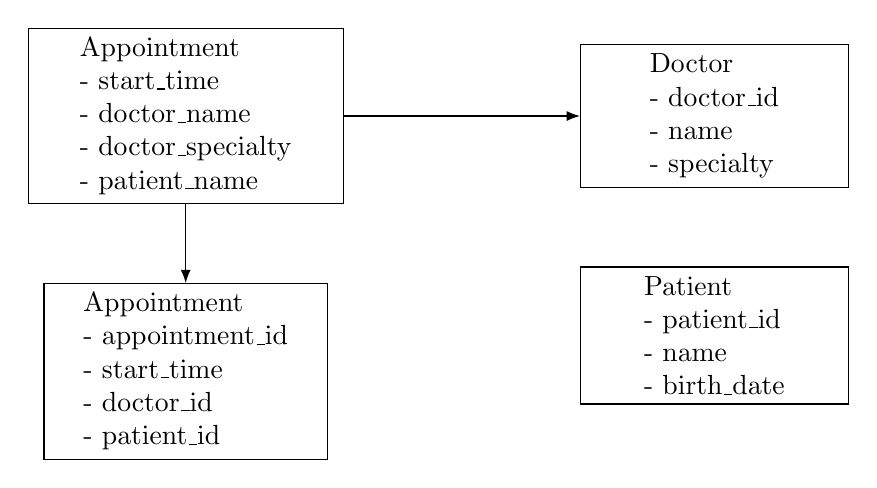
\begin{tikzpicture}[node distance=12mm, >=Latex]
  \node[draw, rectangle, minimum width=4.0cm, minimum height=1.4cm, align=left] (u) {Appointment\\- start\_time\\- doctor\_name\\- doctor\_specialty\\- patient\_name};
  \node[draw, rectangle, minimum width=3.4cm, minimum height=1.1cm, right=30mm of u, align=left] (d) {Doctor\\- doctor\_id\\- name\\- specialty};
  \node[draw, rectangle, minimum width=3.4cm, minimum height=1.1cm, below=10mm of d, align=left] (p) {Patient\\- patient\_id\\- name\\- birth\_date};
  \node[draw, rectangle, minimum width=3.6cm, minimum height=1.1cm, below=10mm of u, align=left] (a) {Appointment\\- appointment\_id\\- start\_time\\- doctor\_id\\- patient\_id};

  \draw[->] (u) -- (d);
  \draw[->] (u) -- (a);
\end{tikzpicture}
\end{document}
